\documentclass[crop,tikz]{standalone}
\usepackage{tikz-3dplot}
\usepackage{pgfplots}
\makeatletter
\usetikzlibrary{3d, arrows.meta, bending, decorations.markings}
\usepgfplotslibrary{polar}
\pgfplotsset{compat=newest}


\makeatletter \newcommand{\pgfplotsdrawaxis}{\pgfplots@draw@axis} \makeatother

\pgfplotsset{axis line on top/.style={
  axis line style=transparent,
  ticklabel style=transparent,
  tick style=transparent,
  axis on top=false,
  after end axis/.append code={
    \pgfplotsset{axis line style=opaque,
      ticklabel style=opaque,
      tick style=opaque,
      grid=none}
    \pgfplotsdrawaxis}
  }
}



\begin{document}


% kepler_2_particles
\tdplotsetmaincoords{70}{110}
  \begin{tikzpicture}[scale=4, tdplot_main_coords]
  	
    \coordinate (O) at (0,0,0);
    \draw[thick] (-1.5,0,0) -- (O);
    \draw[thick] (0,-1,0) -- (O);
    \draw[thick] (0,0,-0.75) -- (O);
    \draw[->, >=latex, thick] (O) -- (1.5,0,0) node[anchor=north east, yshift=1mm]{$X$};
    \draw[->, >=latex, thick] (O) -- (0,1,0) node[right]{$Y$};
    \draw[->, >=latex, thick] (O) -- (0,0,0.75) node[left]{$Z$};
    
    % Define coordinates of the two bodies
    \pgfmathsetmacro{\px}{0.5};
    \pgfmathsetmacro{\py}{-0.9};
    \pgfmathsetmacro{\pz}{0.5};
    \pgfmathsetmacro{\dx}{-1};
    \pgfmathsetmacro{\dy}{0.8};
    \pgfmathsetmacro{\dz}{0.3};
    \coordinate (M1) at (\px,\py,\pz);
    \coordinate (M2) at (\dx,\dy,\dz);
    
    % Draw the positions of each body relative to the origin
    \draw[->,>=stealth] (O) -- (M1) node[pos=0.7, above, yshift=1mm]{$\mathbf{r}_1$};
    \draw[->,>=stealth] (O) -- (M2) node[pos=0.7, above, yshift=1mm]{$\mathbf{r}_2$};
    
    % Draw the projections of both bodies onto the plane
    \draw[dashed] (M1) -- (\px, \py, 0);
    \draw[dashed] (\px, \py, 0) -- (0, \py, 0);
    \draw[dashed] (\px, \py, 0) -- (\px, 0, 0);
    \draw[dashed] (M2) -- (\dx, \dy, 0);
    \draw[dashed] (\dx, \dy, 0) -- (0, \dy, 0);
    \draw[dashed] (\dx, \dy, 0) -- (\dx, 0, 0);
    
    
    %% Draw the vector from body 1 to body 2
    %\draw[->,>=stealth] (M1) -- (M2) node[pos=0.6, above]{$\vec{r}$};
    
	% Draw the bodies
    \fill[fill=blue!50!black!50] (M1) circle (1pt);
    \fill[fill=red!50!black!50] (M2) circle (1pt);    
    
    % Provide the masses
    \node at (M1) [left, xshift=-0.75mm]{$m_1$};
    \node at (M2) [right, xshift=1mm]{$m_2$};
  \end{tikzpicture}

\newpage
% reduced_mass_system
\tdplotsetmaincoords{70}{110}
  \begin{tikzpicture}[scale=4, tdplot_main_coords]
	% Draw a sample trajectory that the particle takes
	\begin{scope}
		% Draw "rings" where the trajectory "passes through the horizontal plane"
		\foreach \t in {49.25, 149.4} {
			\pgfmathsetmacro{\x}{2-cos(\t)^2}
			\pgfmathsetmacro{\y}{-0.35*cos(\t)+\t/180}
			\pgfmathsetmacro{\z}{cos(\t)^2-0.1*sin(\t)}
			\begin{scope}[canvas is xy plane at z=\z]
				\draw[red!80!black!80] (\x,\y) circle (0.2 mm);
 			\end{scope}
 		}
 		
		% Define times at which the trajectory looks like it passes through
		% the planes
		\pgfmathsetmacro{\tlim}{105}
		\pgfmathsetmacro{\tlimTwo}{198}
		\pgfmathsetmacro{\tfinal}{255}
		
		% Flow from the reduced particle through the horizontal plane
		% up until passing through the vertical plane facing the screen
  		\begin{scope}[black, dashed, ->, >=stealth]
  			\pgfplothandlerlineto
  			\pgfplotfunction{\t}{0,1,...,\tlim}
       		{\pgfpointxyz {2-cos(\t)^2}{-0.35*cos(\t)+\t/180}{cos(\t)^2-0.1*sin(\t)}} 
       		\pgfusepath{stroke}
		\end{scope}
  		
  		% Flow in the background until coming back up front
  		\pgfmathsetmacro{\tlimPlusOne}{\tlim+1}
  		\pgfmathsetmacro{\tlimPlusTwo}{\tlim+2}
		\begin{scope}[black!40, dashed, ->, >=stealth]
  			\pgfplothandlerlineto
			\pgfplotfunction{\t}{\tlimPlusOne,\tlimPlusTwo,...,\tlimTwo}
       		{\pgfpointxyz {2-cos(\t)^2}{-0.35*cos(\t)+\t/180}{cos(\t)^2-0.1*sin(\t)}} 
       		\pgfusepath{stroke}
		\end{scope}
		
		% Finish the flow
    		\pgfmathsetmacro{\tlimTwoPlusOne}{\tlimTwo+1}
  		\pgfmathsetmacro{\tlimTwoPlusTwo}{\tlimTwo+2}
		\begin{scope}[black, dashed, ->, >=stealth]
  			\pgfplothandlerlineto
			\pgfplotfunction{\t}{\tlimTwoPlusOne,\tlimTwoPlusTwo,...,\tfinal}
       		{\pgfpointxyz {2-cos(\t)^2}{-0.35*cos(\t)+\t/180}{cos(\t)^2-0.1*sin(\t)}} 
       		\pgfusepath{stroke}
		\end{scope}
    \end{scope}
  
  	
    \coordinate (O) at (0,0,0);
    \draw[thick] (-1.5,0,0) -- (O);
    \draw[thick] (0,-1,0) -- (O);
    \draw[thick] (0,0,-0.725) -- (O);
    \draw[->, >=latex, thick] (O) -- (1.5,0,0) node[anchor=north east, yshift=1mm]{$X$};
    \draw[->, >=latex, thick] (O) -- (0,1.1,0) node[right]{$Y$};
    \draw[->, >=latex, thick] (O) -- (0,0,0.75) node[left]{$Z$};
  	
	% Define the position of the reduced mass particle
  	\coordinate (M) at (1,-0.35,1);
	
	% Draw the position of the reduced mass body relative to the other body
    \draw (O) -- (M) node[pos=0.7, above, yshift=+1mm]{$\mathbf{r}$};
    
    % Draw the reduced mass body
    \fill[fill=green!50!black!50] (M) circle (0.5pt);
    
    % Draw the massive body
    \fill[fill=black!50] (O) circle (1pt);
    
    % Draw the anchor at the origin (mass m1 + m2) and the reduced mass particle
  	\node at (O) [anchor=north west, xshift=1mm, rotate=-6]{$m_1 + m_2$};
    \node at (M) [left]{$\mu^*$};
  \end{tikzpicture}


% Kepler coordinate rotation v2
\tdplotsetmaincoords{70}{110}
\begin{tikzpicture}[scale=2.8, tdplot_main_coords]
  	\coordinate (O) at (0,0,0);
    \draw[thick] (-1.5,0,0) -- (O);
    \draw[thick] (0,-1,0) -- (O);
    \draw[thick] (0,0,-0.75) -- (O);
    \draw[->, >=latex, thick] (O) -- (1.5,0,0) node[anchor=north east, yshift=1mm]{$X$};
    \draw[->, >=latex, thick] (O) -- (0,1,0) node[right]{$Y$};
    \draw[->, >=latex, thick] (O) -- (0,0,0.75) node[left]{$Z$};
    
	\pgfmathsetmacro{\moveRight}{1.2}
    \pgfmathsetmacro{\lengthArrow}{0.54}
    \begin{scope}[shift={({(-0.45/1.25)*\moveRight},\moveRight,0)}]
		\coordinate (O) at (0,0,0);
		\pgfmathsetmacro{\makeArrowStraight}{-0.36*\lengthArrow}
		\draw[->, -{Latex[scale=1]}, very thick, black] (O) -- (\makeArrowStraight, \lengthArrow) node[pos=0.5, above]{\scalebox{1}{$\mathbf{R}$}};
	\end{scope}
    
    	\begin{scope}[shift={(-1.08,3,0)}]
    		\coordinate (O) at (0,0,0);
    		\draw[thick, black!25] (-1.5,0,0) -- (O);
	    \draw[thick, black!25] (0,-1,0) -- (O);
	    \draw[thick, black!25] (0,0,-0.75) -- (O);
    		\draw[->, >=latex, thick, black!25] (0,0,0) -- (1.5,0,0) node[anchor=north east, yshift=1mm]{$X$};
    		\draw[->, >=latex, thick, black!25] (O) -- (0,1,0) node[right]{$Y$};
	    \draw[->, >=latex, thick, black!25] (O) -- (0,0,0.75) node[left]{$Z$};
	    
	    \tdplotsetrotatedcoords{60}{-20}{-90}
	    \tdplotsetrotatedcoords{120}{-30}{-35}%
	    \tdplotsetrotatedcoords{-55}{40}{-15}
	    \begin{scope}[tdplot_rotated_coords]
	    		\begin{scope}[canvas is xy plane at z=0]
	    			\fill[blue!25,fill opacity=0.3] (-1.4,-1.2) rectangle (1.2,1.2);
	    			\node[black, transform shape, scale=0.425, yscale=-1, xscale=-1] at (-0.85,-1) {orbital plane};
	    		\end{scope}
	    		% Draw rotated coordinates
	    		\draw[->, >=latex, thick] (0,0,0) -- (1,0,0) node[left, yshift=-0.5mm]{$x$};
	    		\draw[->, >=latex, thick] (O) -- (0,1,0) node[right]{$y$};
		    \draw[->, >=latex, thick] (O) -- (0,0,0.75) node[anchor=south west, xshift=-1mm]{$z$};
		    
		    % Notes on the directions of x and z
		    \node[align=center] at (0.7,-0.8,1) {Direction of \\ angular momentum};
		    \node[align=center] at (1.5,0,0.2) {Direction of \\ LRL vector};
	    \end{scope}
	    
	    \tdplotcalctransformrotmain
    \end{scope}
\end{tikzpicture}


\newpage
% Kepler coordinate rotation
\tdplotsetmaincoords{70}{110}
  \begin{tikzpicture}[scale=4, tdplot_main_coords]
	% Define the position of the reduced mass particle
	\pgfmathsetmacro{\Mx}{-1}
	\pgfmathsetmacro{\My}{0.75}
	\pgfmathsetmacro{\Mz}{0}
	% Draw a sample trajectory that the particle takes
	\begin{scope}
		% Flow from the reduced particle through the horizontal plane
		% up until passing through the vertical plane facing the screen
  		\begin{scope}[black, dashed, ->, >=stealth]
  			\pgfplothandlerlineto
  			\pgfplotfunction{\t}{0,1,...,360}
       		{\pgfpointxyz {\Mx - sin(\t*2) + \t/180}{\My - 2*sin(\t/2)}{0}} 
       		\pgfusepath{stroke}
       		% Label the trajectory as planar
       		\node at (-1.1, -0.9){planar trajectory};
		\end{scope}
%  		
%  		% Flow in the background until coming back up front
%  		\pgfmathsetmacro{\tlimPlusOne}{\tlim+1}
%  		\pgfmathsetmacro{\tlimPlusTwo}{\tlim+2}
%		\begin{scope}[black!40, dashed, ->, >=stealth]
%  			\pgfplothandlerlineto
%			\pgfplotfunction{\t}{\tlimPlusOne,\tlimPlusTwo,...,\tlimTwo}
%       		{\pgfpointxyz {-0.35*cos(\t)+\t/180}{cos(\t)^2-0.1*sin(\t)}{2-cos(\t)^2}} 
%       		\pgfusepath{stroke}
%		\end{scope}
%		
%		% Finish the flow
%    		\pgfmathsetmacro{\tlimTwoPlusOne}{\tlimTwo+1}
%  		\pgfmathsetmacro{\tlimTwoPlusTwo}{\tlimTwo+2}
%		\begin{scope}[black, dashed, ->, >=stealth]
%  			\pgfplothandlerlineto
%			\pgfplotfunction{\t}{\tlimTwoPlusOne,\tlimTwoPlusTwo,...,\tfinal}
%       		{\pgfpointxyz {-0.35*cos(\t)+\t/180}{cos(\t)^2-0.1*sin(\t)}{2-cos(\t)^2}} 
%       		\pgfusepath{stroke}
%		\end{scope}
    \end{scope}

	\coordinate (O) at (0,0,0);
    \draw[thick] (-1.5,0,0) -- (O);
    \draw[thick] (0,-1,0) -- (O);
    \draw[thick] (0,0,-0.75) -- (O);
    \draw[->, >=latex, thick] (O) -- (1.5,0,0) node[anchor=north east, yshift=1mm]{$x$};
    \draw[->, >=latex, thick] (O) -- (0,1,0) node[right]{$y$};
    \draw[->, >=latex, thick] (O) -- (0,0,0.75) node[left]{$z$};
  	
	% Make coordinate for particle
  	\coordinate (M) at (\Mx, \My, \Mz);
	
	% Draw the (x, y) components
	\draw[dashed] (M) -- (\Mx, 0, 0);
	\draw[dashed] (M) -- (0, \My, 0);
	
    % Draw the position of the reduced mass body relative to the other body
    % with both r and t
    \draw (O) -- (M) node[pos=0.5, above, yshift=0mm]{$r$};
    % Draw the angle
    \tdplotdefinepoints(0,0,0)(0.5,0,0)(\Mx,\My,0)
	\tdplotdrawpolytopearc[->, >=stealth]{0.5}{anchor=north,xshift=-0mm, yshift=-0.5mm}{$\theta$}
    
	% Draw the reduced mass body
    \fill[fill=green!50!black!50] (M) circle (0.5pt);    
	% Draw the massive body
	\fill[fill=black!50] (O) circle (1pt);    
    
    % Draw the anchor at the origin (mass m1 + m2) and the reduced mass particle
  	\node at (O) [anchor=south east, xshift=-1mm, rotate=-6]{$m_1 + m_2$};
    \node at (M) [right]{$\mu^*$};
  \end{tikzpicture}
  
  
  
  
% Polar coordinate system
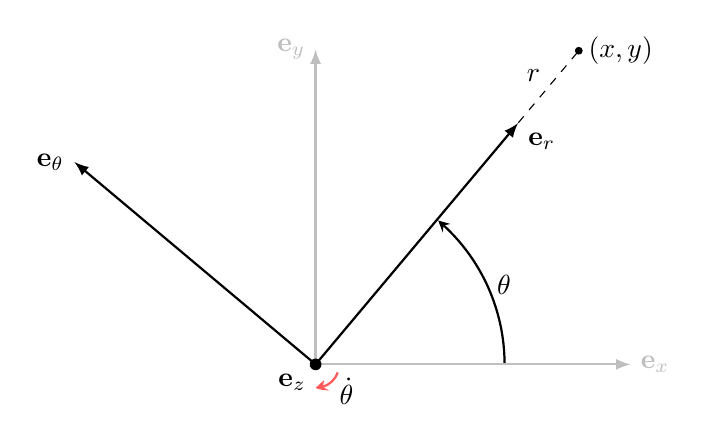
\begin{tikzpicture}[scale=4]
% Draw the polar axes
\pgfmathsetmacro{\radius}{1.3}
\pgfmathsetmacro{\th}{50}
\begin{scope}[rotate=\th]
% Draw the object at (x,y)
\node at (\radius,0) [circle,fill,inner sep=1pt]{};
\node at (\radius, 0)[right]{$(x,y)$};
\draw[thin, dashed] (0,0) -- (\radius,0) node[pos=0.92, left, xshift=-1mm]{$r$};
\draw[->, >=latex, thick] (0,0) -- (1,0) node[anchor=north west]{$\mathbf{e}_r$};
\draw[->, >=latex, thick] (0,0) -- (0,1) node[left]{$\mathbf{e}_\theta$};
\end{scope}

% Draw the angle theta
\pgfmathsetmacro{\rArc}{0.6}
\draw[thick, -{stealth[black]}, black, shorten >=0.5pt] (\rArc,0) arc (0:\th:\rArc) node[pos=0.5, right, black]{$\theta$};
%\draw[thick, path fading=south, shorten >=2pt] (\rArc,0) arc (0:\th:\rArc);

% Draw the normal (x, y) axes
\draw[->, >=latex, thick, black!25] (0,0) -- (1,0) node[right]{$\mathbf{e}_x$};
\draw[->, >=latex, thick, black!25] (0,0) -- (0,1) node[left]{$\mathbf{e}_y$};
\node at (0,0) [circle,fill,inner sep=1.5pt]{};
\node at (0,0) [anchor=north east]{$\mathbf{e}_z$};

% Draw angular velocity
\pgfmathsetmacro{\OmegaArc}{0.075}
\pgfmathsetmacro{\OmegaStartAng}{-20}
\pgfmathsetmacro{\OmegaTotalAng}{-70}
\pgfmathsetmacro{\OmegaAng}{\OmegaStartAng+\OmegaTotalAng}
\draw[thick, -{stealth[bend, red!65]}, red!65] ({\OmegaArc*cos(\OmegaStartAng)},{\OmegaArc*sin(\OmegaStartAng)}) arc (\OmegaStartAng:\OmegaAng:\OmegaArc) node[black, pos=0.8, right, xshift=1mm, yshift=-0.5mm]{$\dot{\theta}$};
\end{tikzpicture}


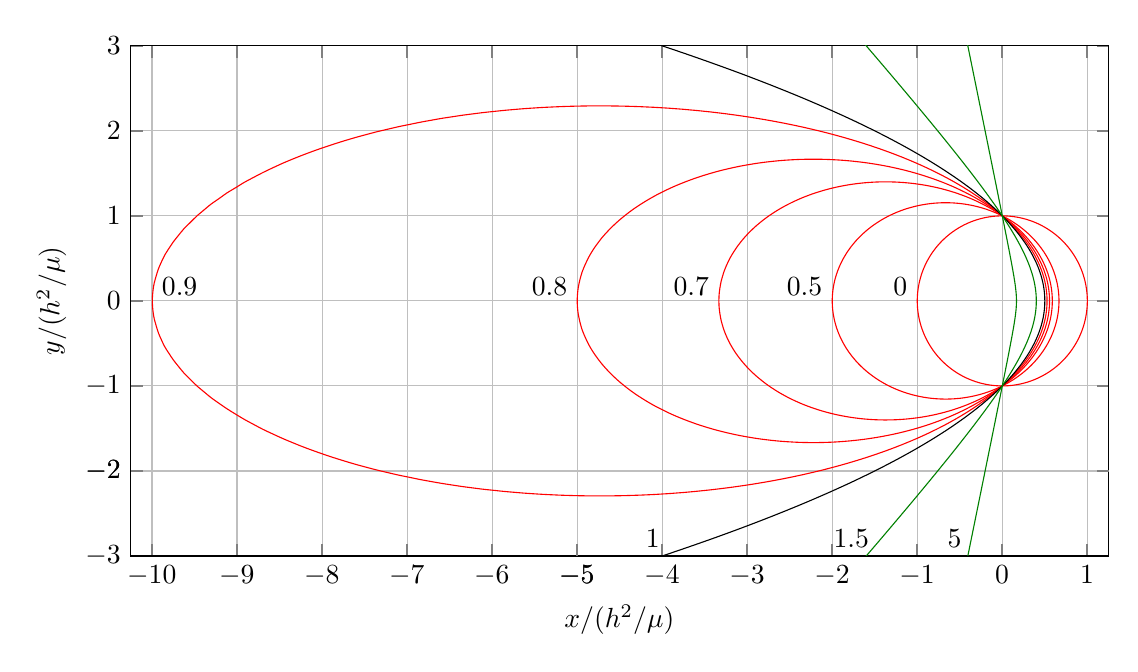
\begin{tikzpicture}
\begin{axis}[width=14cm,
			axis lines=box,
            axis equal image,
            grid=major,
            xmin=-10.25, xmax=1.25,
            ymin=-3, ymax=3,
            xlabel=$x/(h^2/\mu)$, xlabel style={below},
            ylabel=$y/(h^2/\mu)$, ylabel style={above},
            tick style={thick},
            ticklabel style={font=\normalsize},
            xtick={1,0,...,-20}, extra x ticks={-5}, extra x tick style={grid=none},
            ytick={-3,-2,...,3}, minor ytick={-1,1,...,4},extra y ticks={-2}, extra y tick style={grid=none},
            %xmajorticks=false,
            %ymajorticks=false,
            %legend entries={0.5x},
            %        legend style={
            %    at={(0.8,0.937)},
            %    anchor=north,
            %    legend columns=1},
            %    legend cell align={left}
            %axis line on top,
        ]
\addplot[data cs=polar,red,domain=0:360,samples=360,smooth] (x, {1/(1 + 0.000*cos(x)))}) node[pos=0.5, anchor = south east, rotate=0, black,yshift=-0.5mm]{$0$};
\addplot[data cs=polar,red,domain=0:360,samples=500,smooth] (x, {1/(1 + 0.500*cos(x)))}) node[pos=0.5, anchor = south east, rotate=0, black,yshift=-0.5mm]{$0.5$};
\addplot[data cs=polar,red,domain=0:360,samples=500,smooth] (x, {1/(1 + 0.700*cos(x)))}) node[pos=0.5, anchor = south east, rotate=0, black,yshift=-0.5mm]{$0.7$};
\addplot[data cs=polar,red,domain=0:360,samples=500,smooth] (x, {1/(1 + 0.8*cos(x)))}) node[pos=0.5, anchor = south east, rotate=0, black,yshift=-0.5mm]{$0.8$};
\addplot[data cs=polar,red,domain=0:360,samples=750,smooth] (x, {1/(1 + 0.9*cos(x)))}) node[pos=0.5, anchor = south west, rotate=0, black, xshift=0mm,yshift=-0.5mm]{$0.9$};%node[pos=0.441, left, rotate=0, black, xshift=-1mm]{$0.9$};
%\addplot[data cs=polar,red,domain=0:360,samples=360,smooth] (x, {1/(1 + 0.995*cos(x)))}) node[pos=0.9853, above, rotate=0, black, xshift=-3mm]{$0.995$};

\addplot[data cs=polar,black,domain={-acos(-1/1.2)*0.999}:{acos(-1/1.2)*0.999},samples=360,smooth] (x, {1/(1 + cos(x)))}) node[pos=0.07, anchor = south east, rotate=0, black, xshift=1.6mm]{$1$};

%\addplot[data cs=polar,green!50!black,domain={-acos(-1/1.25)*0.999}:{acos(-1/1.25)*0.999},samples=360,smooth] (x, {1/(1 + 1.25*cos(x)))})  node[left, rotate=0, black, yshift=2.2mm] at (axis cs: -2, -3) {$1.25$};
\addplot[data cs=polar,green!50!black,domain={-acos(-1/1.5)*0.999}:{acos(-1/1.5)*0.999},samples=360,smooth] (x, {1/(1 + 1.5*cos(x)))})  node[left, rotate=0, black, yshift=2.2mm] at (axis cs: -1.45, -3) {$1.5$};
\addplot[data cs=polar,green!50!black,domain={-acos(-1/5)*0.999}:{acos(-1/5)*0.999},samples=360,smooth] (x, {1/(1 + 5*cos(x)))})  node[pos=0.4875, left, rotate=0, black, yshift=0.02mm]{$5$};
        
%\legend{$f(x)=\sqrt{x} \; {,} \; x \geq 0$ , $g(x)=0.5x$}
\end{axis}
\end{tikzpicture}



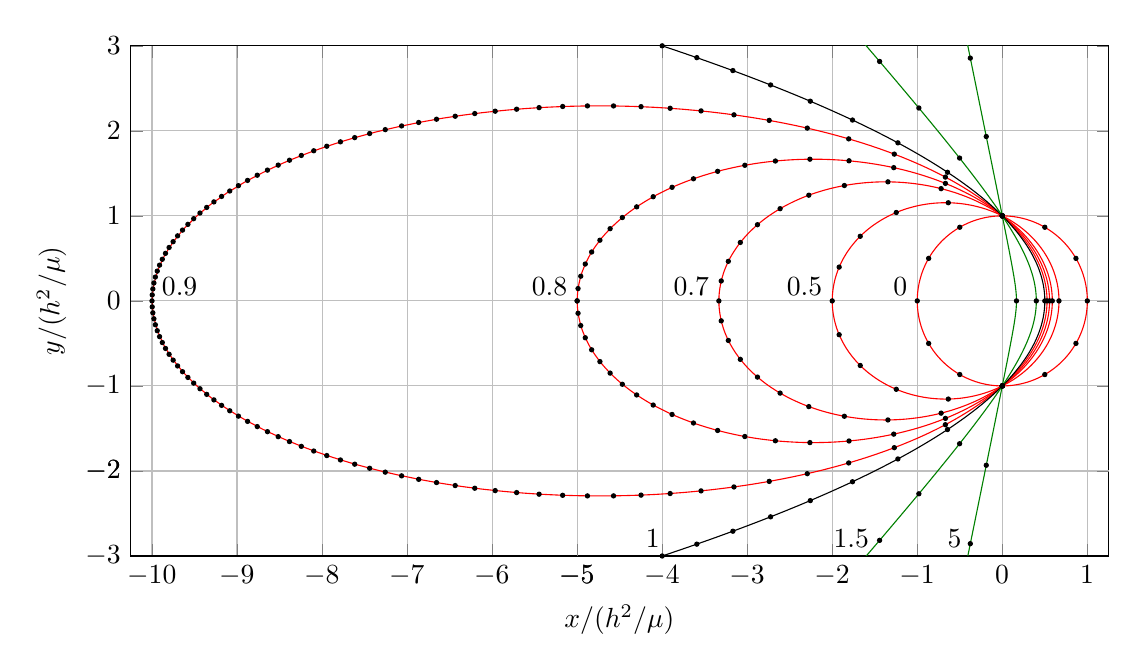
\begin{tikzpicture}
\begin{axis}[width=14cm,
			%axis lines=left,
			axis x line=box,
			axis y line=box,
            axis equal image,
            grid=major,
            xmin=-10.25, xmax=1.25,
            ymin=-3, ymax=3,
            xlabel=$x/(h^2/\mu)$, xlabel style={below},
            ylabel=$y/(h^2/\mu)$, ylabel style={above},
            %tick style={thick},
            ticklabel style={font=\normalsize},
            xtick={1,0,...,-20}, extra x ticks={-5}, extra x tick style={grid=none},
            ytick={-3,-2,...,3}, minor ytick={-1,1,...,4},extra y ticks={-2}, %extra y tick style={grid=none},
            %xmajorticks=false,
            %ymajorticks=false,
            %legend entries={0.5x},
            %        legend style={
            %    at={(0.8,0.937)},
            %    anchor=north,
            %    legend columns=1},
            %    legend cell align={left}
            %axis line on top,
        ]
        
% Marker size
\pgfmathsetmacro{\ms}{0.75}
% e = 0
\addplot[data cs=polar,red,domain=0:360,samples=360,smooth] (x, {1/(1 + 0.000*cos(x)))}) node[pos=0.5, anchor = south east, rotate=0, black, yshift=-0.5mm]{$0$};
\addplot[only marks, draw=black, mark size=\ms] coordinates {    (1,0)    (0.86603,0.5)    (0.5,0.86603)    (6.1232e-17,1)    (-0.5,0.86603)    (-0.86603,0.5)    (-1,0)    (0.86603,-0.5)    (0.5,-0.86603)    (6.1232e-17,-1)    (-0.5,-0.86603)    (-0.86603,-0.5)  };
% e = 0.5
\addplot[data cs=polar,red,domain=0:360,samples=500,smooth] (x, {1/(1 + 0.500*cos(x)))}) node[pos=0.5, anchor = south east, rotate=0, black, yshift=-0.5mm]{$0.5$};
\addplot[only marks, draw=black, mark size=\ms] coordinates {  (0.66667,0)    (0,1)    (-0.63502,1.1544)    (-1.2468,1.0397)    (-1.6707,0.75982)    (-1.9185,0.39753)    (-2,0)    (0,-1)    (-0.63502,-1.1544)    (-1.2468,-1.0397)    (-1.6707,-0.75982)    (-1.9185,-0.39753)  };
% e = 0.7
\addplot[data cs=polar,red,domain=0:360,samples=500,smooth] (x, {1/(1 + 0.700*cos(x)))}) node[pos=0.5, anchor = south east, rotate=0, black, yshift=-0.5mm]{$0.7$};
\addplot[only marks, draw=black, mark size=\ms] coordinates {  (0.58824,0)    (0,1)    (-0.71945,1.3203)    (-1.345,1.4001)    (-1.8574,1.3568)    (-2.2755,1.243)    (-2.613,1.0845)    (-2.8792,0.89611)    (-3.0808,0.68743)    (-3.222,0.46519)    (-3.3056,0.23459)    (-3.3333,0)    (0,-1)    (-0.71945,-1.3203)    (-1.345,-1.4001)    (-1.8574,-1.3568)    (-2.2755,-1.243)    (-2.613,-1.0845)    (-2.8792,-0.89611)    (-3.0808,-0.68743)    (-3.222,-0.46519)    (-3.3056,-0.23459)  };
% e = 0.8
\addplot[data cs=polar,red,domain=0:360,samples=500,smooth] (x, {1/(1 + 0.8*cos(x)))}) node[pos=0.5, anchor = south east, rotate=0, black, yshift=-0.5mm]{$0.8$};
\addplot[only marks, draw=black, mark size=\ms] coordinates {   (0.55556,0)    (0,1)    (-0.66893,1.3817)    (-1.2767,1.5671)    (-1.8026,1.6475)    (-2.2625,1.6665)    (-2.6683,1.645)    (-3.0281,1.595)    (-3.3478,1.5237)    (-3.6319,1.4361)    (-3.8836,1.3357)    (-4.1057,1.225)    (-4.3001,1.1061)    (-4.4685,0.98047)    (-4.6122,0.8494)    (-4.7322,0.71396)    (-4.8294,0.57507)    (-4.9044,0.43353)    (-4.9576,0.29006)    (-4.9894,0.14534)    (-5,2.3769e-08)    (0,-1)    (-0.66893,-1.3817)    (-1.2767,-1.5671)    (-1.8026,-1.6475)    (-2.2625,-1.6665)    (-2.6683,-1.645)    (-3.0281,-1.595)    (-3.3478,-1.5237)    (-3.6319,-1.4361)    (-3.8836,-1.3357)    (-4.1057,-1.225)    (-4.3001,-1.1061)    (-4.4685,-0.98047)    (-4.6122,-0.8494)    (-4.7322,-0.71396)    (-4.8294,-0.57507)    (-4.9044,-0.43353)    (-4.9576,-0.29006)    (-4.9894,-0.14534)    (-5,0)  };
% e = 0.9
\addplot[data cs=polar,red,domain=0:360,samples=750,smooth] (x, {1/(1 + 0.9*cos(x)))}) node[pos=0.5, anchor=south west, rotate=0, black, xshift=0mm, yshift=-0.5mm]{$0.9$}; %node[pos=0.441, left, rotate=0, black, xshift=-1mm]{$0.9$};
\addplot[only marks, draw=black, mark size=\ms] coordinates {   (0.52632,0)    (0,1)    (-0.66931,1.4559)    (-1.2699,1.7261)    (-1.8065,1.9057)    (-2.2935,2.032)    (-2.7409,2.1228)    (-3.1557,2.1882)    (-3.5429,2.2344)    (-3.9062,2.2654)    (-4.2486,2.2843)    (-4.5722,2.293)    (-4.879,2.2933)    (-5.1703,2.2864)    (-5.4475,2.2731)    (-5.7117,2.2545)    (-5.9636,2.231)    (-6.2042,2.2032)    (-6.434,2.1716)    (-6.6537,2.1366)    (-6.8637,2.0985)    (-7.0646,2.0576)    (-7.2567,2.0141)    (-7.4404,1.9683)    (-7.6161,1.9204)    (-7.784,1.8705)    (-7.9445,1.8189)    (-8.0977,1.7655)    (-8.2438,1.7107)    (-8.3832,1.6544)    (-8.5159,1.5968)    (-8.6422,1.538)    (-8.7621,1.4781)    (-8.8759,1.4171)    (-8.9836,1.3552)    (-9.0855,1.2923)    (-9.1815,1.2287)    (-9.2719,1.1643)    (-9.3566,1.0992)    (-9.4358,1.0334)    (-9.5096,0.96703)    (-9.578,0.90012)    (-9.6411,0.83272)    (-9.6989,0.76486)    (-9.7515,0.69659)    (-9.799,0.62795)    (-9.8414,0.55898)    (-9.8787,0.48973)    (-9.911,0.42022)    (-9.9382,0.35051)    (-9.9605,0.28062)    (-9.9778,0.21058)    (-9.9901,0.14045)    (-9.9975,0.070241)    (-10,0)    (0,-1)    (-0.66931,-1.4559)    (-1.2699,-1.7261)    (-1.8065,-1.9057)    (-2.2935,-2.032)    (-2.7409,-2.1228)    (-3.1557,-2.1882)    (-3.5429,-2.2344)    (-3.9062,-2.2654)    (-4.2486,-2.2843)    (-4.5722,-2.293)    (-4.879,-2.2933)    (-5.1703,-2.2864)    (-5.4475,-2.2731)    (-5.7117,-2.2545)    (-5.9636,-2.231)    (-6.2042,-2.2032)    (-6.434,-2.1716)    (-6.6537,-2.1366)    (-6.8637,-2.0985)    (-7.0646,-2.0576)    (-7.2567,-2.0141)    (-7.4404,-1.9683)    (-7.6161,-1.9204)    (-7.784,-1.8705)    (-7.9445,-1.8189)    (-8.0977,-1.7655)    (-8.2438,-1.7107)    (-8.3832,-1.6544)    (-8.5159,-1.5968)    (-8.6422,-1.538)    (-8.7621,-1.4781)    (-8.8759,-1.4171)    (-8.9836,-1.3552)    (-9.0855,-1.2923)    (-9.1815,-1.2287)    (-9.2719,-1.1643)    (-9.3566,-1.0992)    (-9.4358,-1.0334)    (-9.5096,-0.96703)    (-9.578,-0.90012)    (-9.6411,-0.83272)    (-9.6989,-0.76486)    (-9.7515,-0.69659)    (-9.799,-0.62795)    (-9.8414,-0.55898)    (-9.8787,-0.48973)    (-9.911,-0.42022)    (-9.9382,-0.35051)    (-9.9605,-0.28062)    (-9.9778,-0.21058)    (-9.9901,-0.14045)    (-9.9975,-0.070241)  };
% e = 1
\addplot[data cs=polar,black,domain={-acos(-1/1.2)*0.999}:{acos(-1/1.2)*0.999},samples=360,smooth] (x, {1/(1 + cos(x)))}) node[pos=0.07, anchor = south east, rotate=0, black, xshift=1.6mm]{$1$};
%\addplot[only marks, draw=black, mark size=\ms] coordinates {   		 (-6.1971308144716,         -3.65981715785682)         (-5.67992702021268,         -3.51565840781288)          (-5.1436101024248,         -3.35964584515237)         (-4.58502796894654,         -3.18905251413223)         (               -4,                        -3)         (-3.38276711029923,          -2.7866708131027)         ( -2.7249973367406,         -2.53968397118248)         (-2.01383300435906,         -2.24224575118744)         (-1.22773429076116,         -1.85888907187124)        (-0.329355762979384,         -1.28790975070413)         (              0.5,                         0)        (-0.329355762979384,          1.28790975070413)        ( -1.22773429076116,          1.85888907187124)        ( -2.01383300435906,          2.24224575118744)        (  -2.7249973367406,          2.53968397118248)        ( -3.38276711029923,           2.7866708131027)        (                -4,                         3)        ( -4.58502796894654,          3.18905251413223)        (  -5.1436101024248,          3.35964584515237)        ( -5.67992702021268,          3.51565840781288)         ( -6.1971308144716,          3.65981715785682)  };
\addplot[only marks, draw=black, mark size=\ms] coordinates {					(0.5,			 0)     				(0,          1)        (-0.644199211602797,          1.51274532661833)         (-1.22773429076116,          1.85888907187124)         (-1.76157389536461,          2.12676933181039)         (-2.25790158942058,          2.34857471221189)          (-2.7249973367406,          2.53968397118248)         (-3.16852971343876,          2.70870068979161)         (-3.59253555812821,          2.86095632896702)                        (-4,          3)     					(0,                         -1)        (-0.644199211602797,          -1.51274532661833)         (-1.22773429076116,          -1.85888907187124)         (-1.76157389536461,          -2.12676933181039)         (-2.25790158942058,          -2.34857471221189)          (-2.7249973367406,          -2.53968397118248)         (-3.16852971343876,          -2.70870068979161)         (-3.59253555812821,          -2.86095632896702)                        (-4,          -3)};
% e = 1.5
%\addplot[data cs=polar,green!50!black,domain={-acos(-1/1.25)*0.999}:{acos(-1/1.25)*0.999},samples=360,smooth] (x, {1/(1 + 1.25*cos(x)))})  node[left, rotate=0, black, yshift=2.2mm] at (axis cs: -2, -3) {$1.25$};
\addplot[data cs=polar,green!50!black,domain={-acos(-1/1.5)*0.999}:{acos(-1/1.5)*0.999},samples=360,smooth] (x, {1/(1 + 1.5*cos(x)))})  node[left, rotate=0, black, yshift=2.2mm] at (axis cs: -1.45, -3) {$1.5$};
%\addplot[only marks, draw=black, mark size=\ms] coordinates {   		 (-7.95733551093237,         -10.1990681963956)         (-7.16695751152537,         -9.31168472939181)         (-6.37214101433671,         -8.41853012266692)          (-5.5718785437211,         -7.51817290062139)         (-4.76476522141227,         -6.60855734508007)         (-3.94875296745306,         -5.68656938758518)         (-3.12067612357243,         -4.74713626368689)         (-2.27523223547513,         -3.78107773830515)         (-1.40244957256947,         -2.76874154124375)        (-0.480325572003057,         -1.65207976045627)        (0.4               ,          0)        (-0.480325572003057,          1.65207976045627)         (-1.40244957256947,          2.76874154124375)         (-2.27523223547513,          3.78107773830515)         (-3.12067612357243,          4.74713626368689)         (-3.94875296745306,          5.68656938758518)         (-4.76476522141227,          6.60855734508007)          (-5.5718785437211,          7.51817290062139)         (-6.37214101433671,          8.41853012266692)         (-7.16695751152537,          9.31168472939181)         (-7.95733551093237,          10.1990681963956)  };
\addplot[only marks, draw=black, mark size=\ms] coordinates { (0.4,  0) (0,    1) (-0.502090533553359,           1.6796994464829) (-0.981095536305623,          2.26858373729413) (-1.44288702796409,          2.81621462307582) (0,   -1) (-0.502090533553359,           -1.6796994464829) (-0.981095536305623,          -2.26858373729413) (-1.44288702796409,          -2.81621462307582)};
% e = 5
\addplot[data cs=polar,green!50!black,domain={-acos(-1/5)*0.999}:{acos(-1/5)*0.999},samples=360,smooth] (x, {1/(1 + 5*cos(x)))})  node[pos=0.4875, left, rotate=0, black, yshift=0.02mm]{$5$};
%\addplot[only marks, draw=black, mark size=\ms] coordinates {     	(-1.78972017319692,  -9.78629454350939)    (-0.804684087590955, -4.95855184662212)    (0.166666666666667,   0)    (-0.804684087590955,  4.95855184662212)    (-1.78972017319692,   9.78629454350939)  }; 
\addplot[only marks, draw=black, mark size=\ms] coordinates {	(0.166666666666667,                         0)    (0, 											1)    (-0.188434835164092,          1.93301134040144)    (-0.375987051875919,          2.85528647162408)    (-0.562964270032889,          3.77305355969628)    (-0.74957275505812,          4.68832071360218)    (-0.935927901637677,          5.60199463636931)    (-1.12209893486353,          6.51456321018991)    (-1.30813031129068,          7.42631947767708)    (-1.49405218909881,          8.33745336064982)    (0, 											-1)    (-0.188434835164092,          -1.93301134040144)    (-0.375987051875919,          -2.85528647162408)    (-0.562964270032889,          -3.77305355969628)    (-0.74957275505812,          -4.68832071360218)    (-0.935927901637677,          -5.60199463636931)    (-1.12209893486353,          -6.51456321018991)    (-1.30813031129068,          -7.42631947767708)    (-1.49405218909881,          -8.33745336064982)}; 

\end{axis}
\end{tikzpicture}


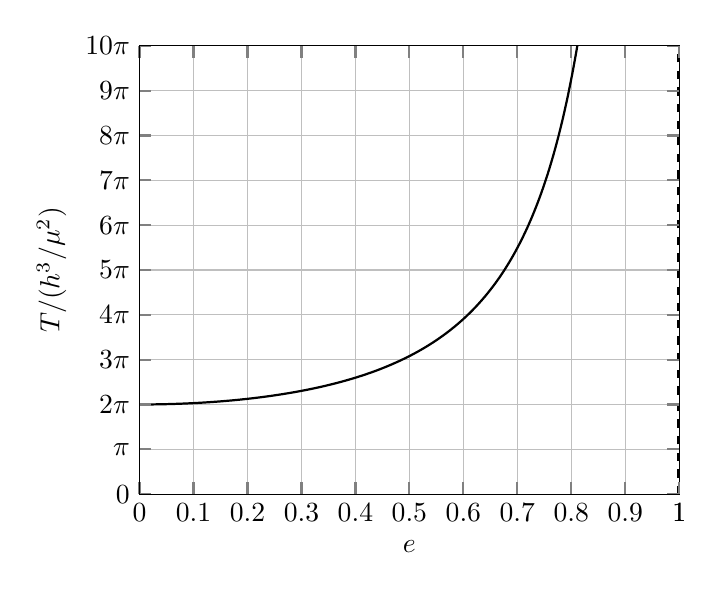
\begin{tikzpicture}
\begin{axis}[%width=14cm,
			%axis lines=left,
			axis x line=box,
			axis y line=box,
%            axis equal image,
            grid=major,
            xmin=0, xmax=1,
            ymin=0, ymax=10*pi,
            xlabel=$e$, xlabel style={below},
            ylabel=$T/(h^3/\mu^2)$,  y label style={above},
            tick style={thick},
            ticklabel style={font=\normalsize},
            xtick={0,0.1,...,1}, extra x ticks={1,1.5,2}, extra x tick style={grid=none},
            ytick={0,pi,2*pi,3*pi,4*pi,5*pi,6*pi,7*pi,8*pi,9*pi,10*pi}, 
            yticklabels={$0$,$\pi$,$2\pi$,$3\pi$,$4\pi$,$5\pi$,$6\pi$,$7\pi$,$8\pi$,$9\pi$,$10\pi$}, 
%            minor ytick={0},
%            extra y ticks={2*pi}, extra y tick style={grid=none,yticklabels={$2\pi$}},
            %xmajorticks=false,
            %ymajorticks=false,
            %legend entries={0.5x},
            %        legend style={
            %    at={(0.8,0.937)},
            %    anchor=north,
            %    legend columns=1},
            %    legend cell align={left}
            axis line on top,
            %label style={font=\large}
        ]
\addplot[black,domain=0:0.95,samples=360,smooth,thick]{2*pi/(1 - x^2)^1.5} node[pos=0.5, anchor = south east, rotate=0, black]{$0$};
\draw [dashed, ultra thick, black] (1,0) -- (1,100);
%\node[below left] at (axis cs:0,0) {$0$};
\end{axis}
\end{tikzpicture}



\end{document}

% GRAVEYARD
%\newpage
%% kepler_solution
%  \begin{tikzpicture}[scale=4]
%    \coordinate (O) at (0,0);
%    \draw[thick] (-0.1,0) -- (O);
%    \draw[thick] (0,-0.1) -- (O);
%    \draw[->, >=latex, thick] (O) -- (1,0) node[right]{$x$};
%    \draw[->, >=latex, thick] (O) -- (0,1) node[left]{$y$};
%    
%    % Define coordinates of the two bodies
%    \pgfmathsetmacro{\px}{0.85};
%    \pgfmathsetmacro{\py}{0.25};
%    \pgfmathsetmacro{\dx}{0.4};
%    \pgfmathsetmacro{\dy}{0.85};
%    \coordinate (M1) at (\px,\py);
%    \coordinate (M2) at (\dx,\dy);
%    
%    % Draw the bodies
%    \fill[fill=blue!50!black!50] (M1) circle (1pt);
%    \fill[fill=red!50!black!50] (M2) circle (1pt);
%    
%    % Draw the positions of each body relative to the origin
%    \draw[->,>=stealth] (O) -- (M1) node[pos=0.6, below, yshift=0mm]{$\mathbf{r}_1$};
%    \draw[->,>=stealth] (O) -- (M2) node[pos=0.6, left, yshift=-1mm]{$\mathbf{r}_2$};
%    
%    % Draw the vector from body 1 to body 2
%    \draw[->,>=stealth] (M1) -- (M2) node[pos=0.55, right]{$\mathbf{r}$};
%    
%    % Provide the masses
%    \node at (M1) [right, xshift=1mm]{$m_1$};
%    \node at (M2) [left, xshift=-1mm]{$m_2$};
%  \end{tikzpicture}




%\newpage
%% Kepler cylindrical coordinates
%\tdplotsetmaincoords{70}{110}
%  \begin{tikzpicture}[scale=4, tdplot_main_coords]
%	\coordinate (O) at (0,0,0);
%  	\pgfmathsetmacro{\x}{1.5}
%  	\pgfmathsetmacro{\y}{1}
%
%%	% Draw grid to show plane
%%	\begin{scope}[canvas is xy plane at z=0]
%%		\draw[step=0.25,black!20,thin,xshift=0.5cm,yshift=0.5cm] (-1.5*\x,-\y) grid (\x,\y);
%%	\end{scope}    	
%  	
%    \draw[->, >=latex, thick] (O) -- (\x,0,0) node[anchor=north east, yshift=1mm]{$\hat{\mathbf{e}}_x$};
%    \draw[->, >=latex, thick] (O) -- (0,\y,0) node[right]{$\hat{\mathbf{e}}_y$};
%    \draw[->, >=latex, thick] (O) -- (0,0,0.75) node[left]{$\hat{\mathbf{e}}_z$};
%    
%    % Draw polar basis
%    \pgfmathsetmacro{\t}{55}
%    \pgfmathsetmacro{\cost}{cos(\t)}
%    \pgfmathsetmacro{\sint}{sin(\t)}
%    
%    \draw[->, >=latex, thick] (O) -- (\x*\cost,\y*\sint,0) node[anchor=north east, yshift=1mm]{$\hat{\mathbf{e}}_r$};
%    \draw[->, >=latex, thick] (O) -- (-\x*\sint,\y*\cost,0) node[right]{$\hat{\mathbf{e}}_\theta$};
%    
%    \tdplotdefinepoints(0,0,0)(0.5,0,0)(\x*\cost,\y*\sint,0)
%	\tdplotdrawpolytopearc[->, >=stealth]{0.5}{anchor=north,xshift=-0mm, yshift=-0.5mm}{$\theta$}
%  \end{tikzpicture}





%\newpage
%\begin{tikzpicture}[scale=4]
%	\draw[->, >=latex, thick] (0,0) -- (1,0) node[right]{$\hat{\mathbf{e}}_x$};
%	\draw[->, >=latex, thick] (0,0) -- (0,1) node[left]{$\hat{\mathbf{e}}_y$};
%	
%	% Draw polar basis
%    \pgfmathsetmacro{\t}{55}
%    \pgfmathsetmacro{\cost}{cos(\t)}
%    \pgfmathsetmacro{\sint}{sin(\t)}
%    
%    \draw[->, >=latex, thick] (0,0) -- (\cost,\sint) node[anchor=south west, yshift=0mm]{$\hat{\mathbf{e}}_r$};
%    \draw[->, >=latex, thick] (0,0) -- (-\sint,\cost) node[left]{$\hat{\mathbf{e}}_\theta$};
%\end{tikzpicture}









%\newpage
%% Kepler coordinate rotation
%\tdplotsetmaincoords{70}{110}
%  \begin{tikzpicture}[scale=4, tdplot_main_coords]
%  	\coordinate (O) at (0,0,0);
%    \draw[thick] (-1.5,0,0) -- (O);
%    \draw[thick] (0,-1,0) -- (O);
%    \draw[thick] (0,0,-0.75) -- (O);
%    \draw[->, >=latex, thick] (O) -- (1.5,0,0) node[anchor=north east, yshift=1mm]{$X$};
%    \draw[->, >=latex, thick] (O) -- (0,1,0) node[right]{$Y$};
%    \draw[->, >=latex, thick] (O) -- (0,0,0.75) node[left]{$Z$};
%    
%    	\tdplotsetrotatedcoords{60}{-20}{-90}
%    \begin{scope}[tdplot_rotated_coords]
%%    		\draw[thick, black!50] (-1.5,0,0) -- (O);
%%	    \draw[thick, black!50] (0,-1,0) -- (O);
%%	    \draw[thick, black!50] (0,0,-0.75) -- (O);
%    		\draw[->, >=latex, thick, black!50] (O) -- (1,0,0) node[anchor=north east, yshift=1mm]{$x$};
%    		\draw[->, >=latex, thick, black!50] (O) -- (0,1,0) node[right]{$y$};
%	    \draw[->, >=latex, thick, black!50] (O) -- (0,0,1) node[left]{$z$};
%    \end{scope}
%  \end{tikzpicture}










%\begin{tikzpicture}
%\begin{axis}[width=14cm,
%			axis lines=middle,
%			x axis line style={-},
%            %axis equal image,
%            grid=major,
%            xmin=0, xmax=1,
%            ymin=0, ymax=100,
%            xlabel=$e$,
%            ylabel=$\displaystyle\frac{T}{h^3/\mu^2}$, 
%            x label style={at={(axis description cs:0.5,-0.05)},anchor=north},
%		    y label style={at={(axis description cs:-0.115,.5)},rotate=0,anchor=south},
%		    tick style={thick},
%            ticklabel style={font=\normalsize},
%            xtick={0,0.1,...,1}, extra x ticks={0,1}, extra x tick style={grid=none},
%            ytick={0,10,...,100}, extra y ticks={0}, %minor ytick={-1,1,...,4}, extra y tick style={grid=none},
%            axis line on top,
%            label style={font=\large}
%        ]
%\addplot[black,domain=0:0.95,samples=360,smooth]{2*pi/(1 - x^2)^1.5} node[pos=0.5, anchor = south east, rotate=0, black]{$0$};
%\draw [dashed] (1,0) -- (1,100);
%\node[below left] at (axis cs:0,0) {$0$};
%\end{axis}
%\end{tikzpicture}